\subsubsection{Overview}

The instruction planner is controlling the software for 
controlling the robot \\

\subsubsection{Previous implementation}
Shortly describe what the previous team did and why they designed the instruction planner and what 
there intention was. 

\subsubsection{Design}

Describe the overall design of the instruction planner. Which ports are used and connected to other components. What are the tasks of the component and what purpose do they fulfill. 

\begin{figure}[h]
\centering
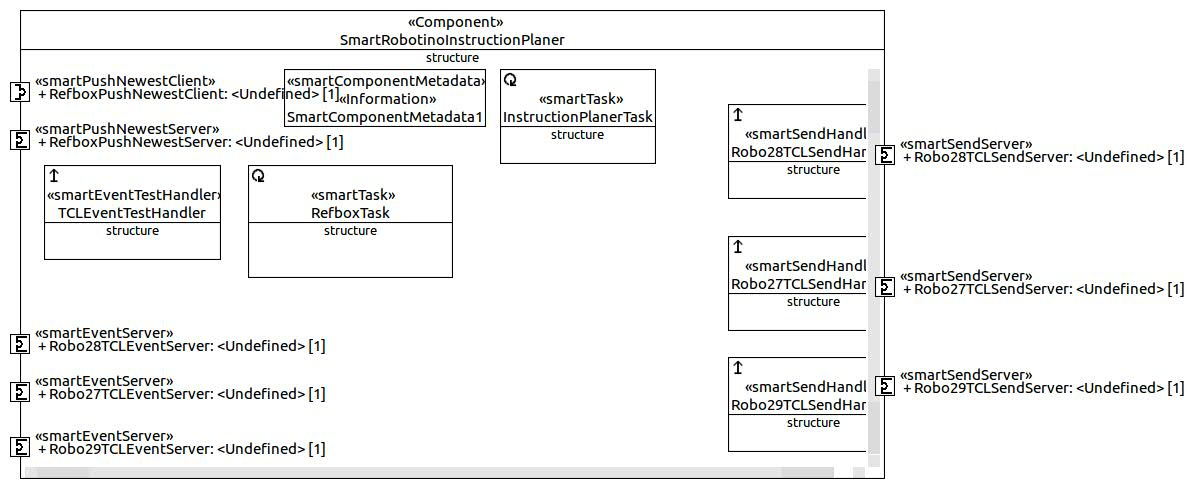
\includegraphics[scale=0.25]{pic/SmartRobotinoInstructionPlaner.JPG}
\caption{Model of InstructionPlanner}
\end{figure}


\subsubsection{Communication Objects}

Describe the messages which are processed by the instruction planner. 

\begin{itemize}

\item CommRefbox \\

Describes the messages which come from the Refbox. This means that in this CommunicationObjecs the 
Phases and States of the running tournament are encoded.

\item MachineInfo \\

The MachineInfo communication object is used to handover the information of detected MPS stations to the SmartRefBoxServer component. 

\item MachineReport \\

\item RobotInfo \\

The RobotInfo is used to send the current state of the robot from the point of the refbox. This message is send from SmartRefboxServer to InstructionPlanner. 

\end{itemize}


\subsubsection{Statemachine}

Describe the state machine with a diagram with states
and transitions

\subsubsection{Maintenance Modes}

Describe how to team and the robot can react to failures and the system. How to set the robot into maintenance mode and how the robot can return to the game. 


\subsubsection{Outcome}

Multiple robots and Production phase







